\documentclass[a4paper]{article}

\usepackage{amsmath,amssymb,amsfonts}
\usepackage{amssymb, amsmath}
\usepackage{ascmac}

\DeclareMathOperator{\Bern}{\rm Bern}
\DeclareMathOperator{\Bin}{\rm Bin}
\DeclareMathOperator{\Po}{\rm Po}
\DeclareMathOperator{\Cat}{\rm Cat}
\DeclareMathOperator{\Mult}{\rm Mult}
\DeclareMathOperator{\Beta}{\rm Beta}
\DeclareMathOperator{\Dir}{\rm Dir}
\DeclareMathOperator{\N}{\rm N}
\DeclareMathOperator{\InvW}{\mathcal{IW}}
\DeclareMathOperator{\NIW}{\mathcal{NIW}}

\newcommand{\relmiddle}[1]{\mathrel{}\middle#1\mathrel{}}

\newcommand{\proptoas}[1]{\overset{#1}{\propto}}

\usepackage{braket}
\usepackage{url}

\usepackage[dvipdfmx]{graphicx}

\title{Sample of GMM parameters estimation using Gibbs sampling method}
\author{Ryo Ozaki\\Ritsumeikan University\\Graduate School of Information Science and Engineering\\Emergent Systems Laboratory\\ryo.ozaki@em.ci.ritsumei.ac.jp}
\begin{document}
\maketitle
\section{Graphical model}
This section shows the graphical model of Gaussian mixture model (GMM) which were used this paper.
\begin{figure}[ht]
	\begin{center}
		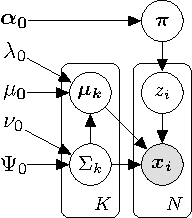
\includegraphics[width=5cm]{fig/GMM_graphical_model.pdf}
		\caption{Graphical model of GMM.}
	\end{center}
\end{figure}

The probabilistic generative process of GMM is shown below.
\begin{eqnarray}
	\lambda &=& \Set{\alpha_0, \lambda_0, \boldsymbol{\mu_0}, \nu_0, \Psi_0}\\
	\theta &=& \Set{\boldsymbol{\pi}, z_{1:N}, \boldsymbol{\mu_{1:K}}, \Sigma_{1:K}}\\
	\nonumber \\
	\boldsymbol{\pi} &\sim& \Dir(\boldsymbol{\pi} | \boldsymbol{\alpha_0})\\
	(\boldsymbol{\mu_k}, \Sigma_k) &\sim& \NIW(\boldsymbol{\mu}, \Sigma | \boldsymbol{\mu_0}, \lambda_0, \Psi_0, \nu_0) \\
	z_i &\sim& \Cat(z | \boldsymbol{\pi}) \\
	\boldsymbol{x_i} &\sim& \N(\boldsymbol{x} | \boldsymbol{\mu}_{z_i}, \Sigma_{z_i})\\
	\nonumber \\
	k &=& 1, 2, \ldots, K\\
	i &=& 1, 2, \ldots, N
\end{eqnarray}
Here, $\lambda$ represents the set of hyperparameters, $\theta$ represents the set of parameters, $\Dir$ represents the Dirichlet distribution, $\N$ represents the normal distribution, $\NIW$ represents the normal-inverse-Wishart distribution, $\Cat$ represents the categorical distribution.

\section{Posterior distribution}
This section shows posterior distributions of the $\theta$.

\subsection{Posterior distribution of $z_i$}
The posterior distribution of $z_i$ is represented as follows.
\begin{eqnarray}
	p(z_i = k | x_i, \boldsymbol{\pi}, \boldsymbol{\mu_{1:K}}, \Sigma_{1:K}) &\proptoas{z_i}& p(x_i | z_i = k, \boldsymbol{\mu_k}, \Sigma_k) p(z_i = k | \boldsymbol{\pi})\\
	&=& \N(\boldsymbol{x_i} | \boldsymbol{\mu_k}, \Sigma_k) \Cat(z_i = k | \boldsymbol{\pi})\\
	&=& \Cat(z_i = k | \boldsymbol{\pi^*})\\
	\nonumber \\
	\pi^{-}_{k} &=& \N(\boldsymbol{x_i} | \boldsymbol{\mu_k}, \Sigma_k) \times \pi_k \\
	\nonumber \\
	\pi^*_k &=& \frac{\pi^{-}_k}{\sum_{l = 1}^{K}{\pi^{-}_l}}
\end{eqnarray}

\subsection{Posterior distribution of $\boldsymbol{\pi}$}
The posterior distribution of $\boldsymbol{\pi}$ is represented as follows.
\begin{eqnarray}
	p(\boldsymbol{\pi} | \boldsymbol{\alpha_0}, z_{1:N}) &\proptoas{\boldsymbol{\pi}}& p(z_{1:N} | \boldsymbol{\pi}) p(\boldsymbol{\pi} | \boldsymbol{\alpha_0})\\
	&=& \prod_{i=1}^{N}{\left\{ p(z_i | \boldsymbol{\pi}) \right\} } p(\boldsymbol{\pi} | \boldsymbol{\alpha_0})\\
	&=& \prod_{i=1}^{N}{\left\{ \Cat(z_i | \boldsymbol{\pi}) \right\} } \Dir(\boldsymbol{\pi} | \boldsymbol{\alpha_0})\\
	&=& \Mult(\boldsymbol{m} | \boldsymbol{\pi}) \Dir(\boldsymbol{\pi} | \boldsymbol{\alpha_0})\\
	&=& \Dir(\boldsymbol{\pi} | \boldsymbol{\alpha^*})\\
	\nonumber \\
	m_k &=& \sum_{i=1}^{N}{\delta(z_i = k)}\\
	\delta(\text{CONDITION}) &=&
	\left\{
	\begin{array}{ll}
		0 & (\text{CONDITION is false})\\
		1 & (\text{CONDITION is true})
	\end{array}
	\right.\\
	\nonumber\\
	\boldsymbol{\alpha^*} &=& \boldsymbol{m} + \boldsymbol{\alpha_0}
\end{eqnarray}
Here, $\Mult$ represents multinomial distribution.

\subsection{Posterior distribution of $\boldsymbol{\mu_k}$ and $\Sigma_k$}
The posterior distribution of $\boldsymbol{\mu_k}$ and $\Sigma_k$ is represented as follows.
\begin{eqnarray}
	\lefteqn{
		p(\boldsymbol{\mu_k}, \Sigma_k | \boldsymbol{\mu_0}, \lambda_0, \Psi_0, \nu_0, \boldsymbol{x_{1:N}}, z_{1:N})
	}\nonumber \\
	&\proptoas{\boldsymbol{\mu_k}, \Sigma_k}& p(\boldsymbol{x^{k}_{1:M}} | \boldsymbol{\mu_k}, \Sigma_k) p(\boldsymbol{\mu_k}, \Sigma_k | \boldsymbol{\mu_0}, \lambda_0, \Psi_0, \nu_0)\\
	&=& \prod_{i=1}^{M}{\left\{ p(z_i | \boldsymbol{\mu_k}, \Sigma_k) \right\}} p(\boldsymbol{\mu_k}, \Sigma_k | \boldsymbol{\mu_0}, \lambda_0, \Psi_0, \nu_0) \\
	&=& \prod_{i=1}^{M}{\left\{ \N(z_i | \boldsymbol{\mu_k}, \Sigma_k) \right\}} \NIW(\boldsymbol{\mu_k}, \Sigma_k | \boldsymbol{\mu_0}, \lambda_0, \Psi_0, \nu_0) \\
	&=& \NIW(\boldsymbol{\mu_k}, \Sigma_k | \boldsymbol{\mu^*}, \lambda^*, \Psi^*, \nu^*) \\
	\nonumber \\
	\boldsymbol{x^{k}_{1:M_k}} &=& \Set{ \boldsymbol{x_i} | z_i = k, i=1, \ldots, N }\\
	M_k &=& \sum_{i=1}^{N}{\delta(z_i = k)} \\
	\boldsymbol{\bar{x}^k} &=& \frac{1}{M_k} \sum_{i=1}^{M_k}{\boldsymbol{x_i^k}} \\
	S^k &=& \sum_{i=1}^{M_k}{\left( \boldsymbol{x_i^k} - \boldsymbol{\bar{x}^k} \right) \left( \boldsymbol{x_i^k} - \boldsymbol{\bar{x}^k} \right)^T} \\
	\nonumber \\
	\lambda^* &=& M_k + \lambda_0 \\
	\boldsymbol{\mu^*} &=& \frac{M_k \cdot \boldsymbol{\bar{x}^k} + \lambda_0 \cdot \boldsymbol{\mu_0}}{M_k + \lambda_0}\\
	\nu^* &=& M_k + \nu_0\\
	\Psi^* &=& S^k + \frac{M_k \lambda_0}{M_k + \lambda_0} \left( \boldsymbol{\bar{x}^k} - \boldsymbol{\mu_0} \right) \left( \boldsymbol{\bar{x}^k} - \boldsymbol{\mu_0} \right)^T + \Psi_0
\end{eqnarray}

\section{Experiments}
This section shows results of experiments.

\subsection{Truth parameters}
Parameters which were used in this experiments represented follows.
\begin{eqnarray}
	\boldsymbol{\pi^*} &=& \left[ \begin{array}{ccc}
		0.7 & 0.2 & 0.1
	\end{array}
	\right]\\
	\boldsymbol{\mu^*_{1:3}} &=& 
	\left[\begin{array}{c}
		3\\
		0
	\end{array}\right]
	, 
	\left[\begin{array}{c}
		-3\\
		0
	\end{array}\right]
	, 
	\left[\begin{array}{c}
		0\\
		5
	\end{array}\right]\\
	\Sigma^*_{1:3} &=& 
	\left[\begin{array}{cc}
		1 & 0\\
		0 & 1
	\end{array}\right]
	, 
	\left[\begin{array}{cc}
		1 & 0\\
		0 & 1
	\end{array}\right]
	, \left[\begin{array}{cc}
		1 & 0\\
		0 & 1
	\end{array}\right]
\end{eqnarray}

\subsection{Hyperparameters}
Hyperparameters which were used in this experiments represented follows.
\begin{eqnarray}
	\boldsymbol{\alpha_0} &=& \left[\begin{array}{cccc} 1 & 1 & 1 & 1\end{array}\right]\\
	\nu_0 &=& 2\\
	\Psi_0 &=& \left[\begin{array}{cc}
		1 & 0\\
		0 & 1
	\end{array}\right]\\
	\boldsymbol{\mu_0} &=& \left[\begin{array}{c}
		0\\
		0
	\end{array}\right]\\
	\lambda_0 &=& 1
\end{eqnarray}

\subsection{Experiment 1}
This section shows a clustering result of the dataset which has 300 observations.
Figure \ref{fig:ex1_truth} shows the dataset which are used in this experiment.
In addition, we set $K = 4$ which is a number of clusters.
We did Gibbs sampling 150 steps.
\begin{figure}[h]
	\begin{center}
		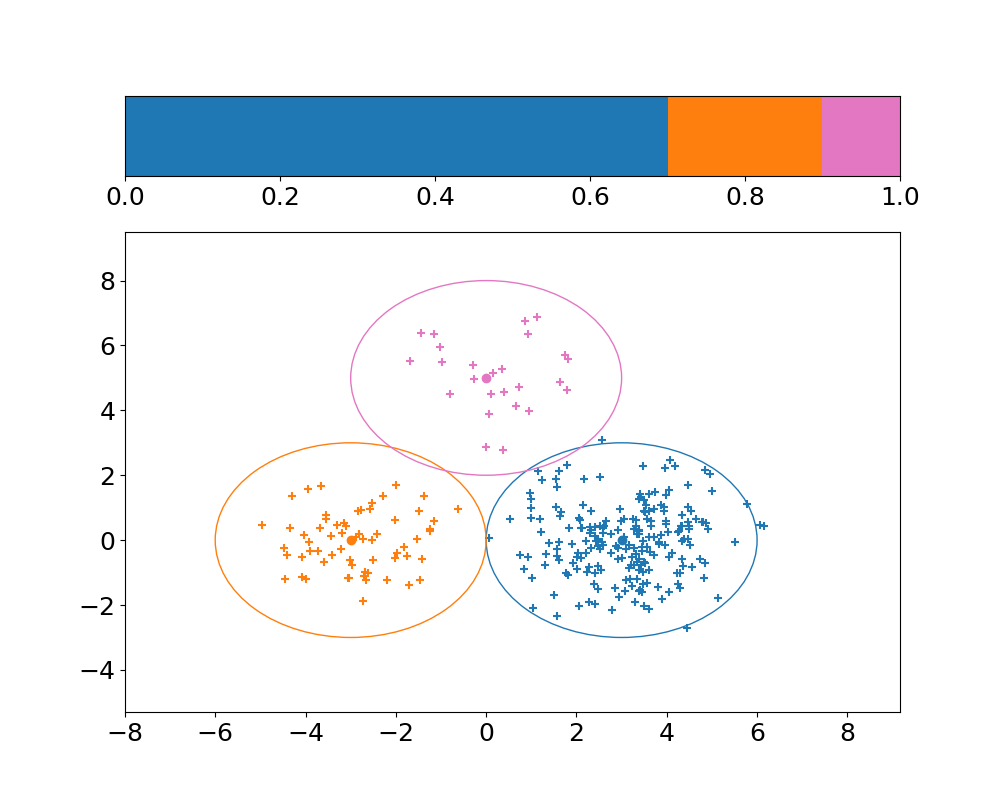
\includegraphics[width=11cm]{fig/ex1/truth.png}
		\caption{Truth data (300 points)}
		\label{fig:ex1_truth}
	\end{center}
\end{figure}

Figure \ref{fig:ex1_result} shows a result at 150-th step in Gibbs sampling.
In addition, you can see the process of Gibbs sampling at the file named ``GMM\_Gibbs\_result1.gif'' which in this directory.
Also, you can see the stochastic behavior of Gibbs sampling.
\begin{figure}[h]
	\begin{center}
		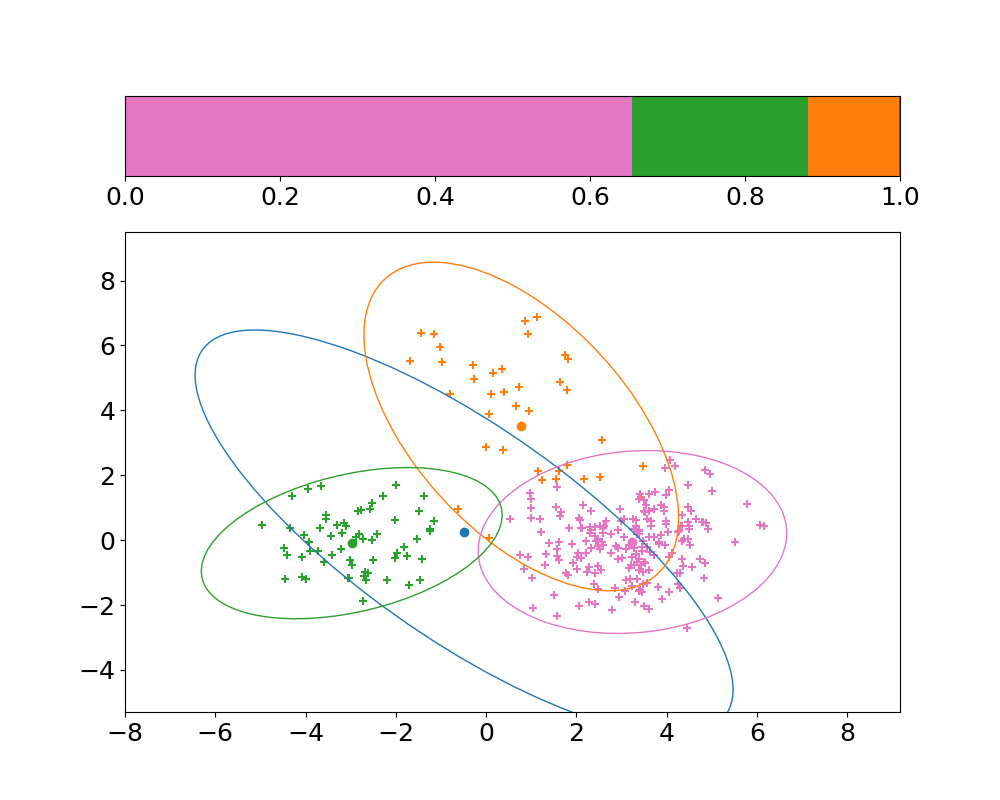
\includegraphics[width=11cm]{fig/ex1/final.png}
		\caption{Result at 150-th step in Gibbs sampling}
		\label{fig:ex1_result}
	\end{center}
\end{figure}

\subsection{Experiment 2}
This section shows a clustering result of the dataset which has 3000 observations.
Figure \ref{fig:ex2_truth} shows the dataset which are used in this experiment.
Other conditions are same as is experiment 1.
\begin{figure}[h]
	\begin{center}
		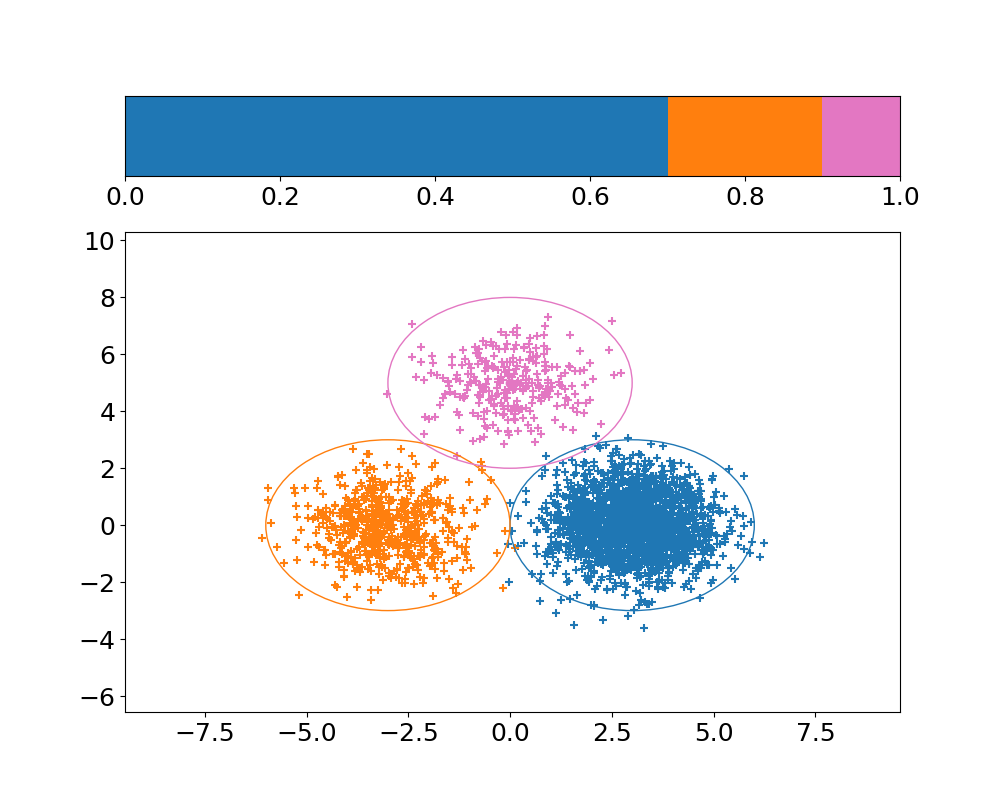
\includegraphics[width=11cm]{fig/ex2/truth.png}
		\caption{Truth data (3000 points)}
		\label{fig:ex2_truth}
	\end{center}
\end{figure}

Figure \ref{fig:ex2_result} shows a result at 150-th step in Gibbs sampling.
In addition, you can see the process of Gibbs sampling at the file named ``GMM\_Gibbs\_result2.gif'' which in this directory.
\begin{figure}[h]
	\begin{center}
		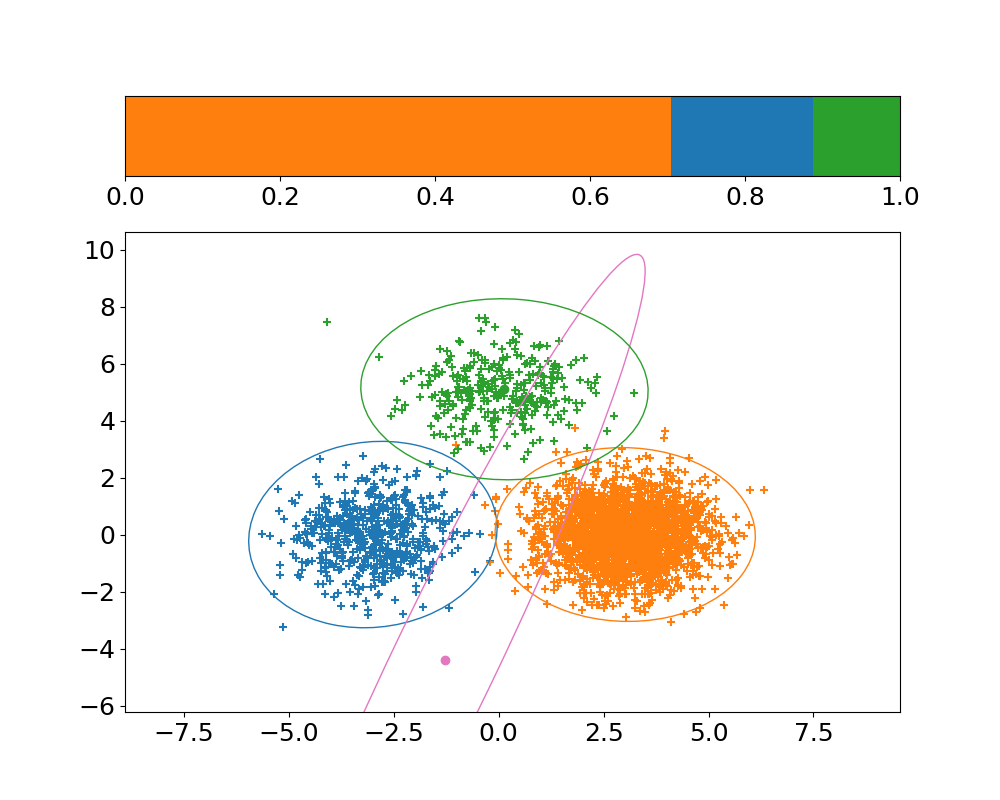
\includegraphics[width=11cm]{fig/ex2/final.png}
		\caption{Result at 150-th step in Gibbs sampling}
		\label{fig:ex2_result}
	\end{center}
\end{figure}

\newpage
\section{Summary}
This paper derived the posterior distributions of parameters $\theta$.
In addition, we estimated the parameters of synthesis dataset which has 300 and 3000 observations.
Also, we showed the stochastic behavior of Gibbs sampling into ``GMM\_Gibbs\_result1.gif'' and ``GMM\_Gibbs\_result2.gif.''

You can the same experiment on your computer using this GitHub repository.
If you want to do, please run following commands.
\begin{enumerate}
	\item \verb|git clone https://github.com/RyoOzaki/GibbsSampling|\\
		Clone this repository to your computer.
	\item \verb|cd GibbsSampling/GMM|\\
		Change directory to ``GMM'' in ``GibbsSampling''.
	\item \verb|python GMM_Gibbs.py|\\
		Run Gibbs sampling. You can get result in ``tmp'' directory.
	\item \verb|sh make_gif.sh|\\
		Convert images in ``fig'' directory to ``result.gif.''
\end{enumerate}


\end{document}
